%%%%%%%%%%%%%%%%%%%%%%%%%%%%%%%%%%%%%%%%%%%%%%%%%%%%%%%%%%%%
\section{Case Definition and Specifications}

This paper sets the proposed case to building a 70,000 \gls{MTHM} capacity borehole
 repository at the Clinton Power Plant in Illinois. The base case is to build a
  standalone borehole repository at a location similar to that of Yucca Mountain with
   the same capacity. The borehole design follows the Sandia Report Reference Design
    and Operations for Deep Borehole Radioactive Waste \cite{arnold_reference_2011}.
     However,the difference in design of borehole will not contribute directly
     to the analysis for the design is the same for both case. The design will
     affect the necessary repacking facility to repack the individual rods into
     a emplacement canister.

\subsection{Proposed Case Methodology and Definition}
 In order to minimize transport cost, a central location is preferred. A metric 
 for representg the spent fuel transport burden, mass distance, is the product 
 of the waste volume and the distance it has to travel. This results in a 
 metric in units of $MTHM\cdot km$. 
 
 This distance analysis was completed using the Haversine formula 
 \cite{shumaker_astronomical_1984}. First, the 
 coordinates of each power plant were obtained by scraping public data 
 \cite{wikipedia}.  The distance between each storage site (i.e. reactors and 
 \gls{ISFSI}) was then calculated by using the Havershine formula on the 
 geographical coordinates of both sites. 

 \begin{align} 
         \Phi_1,\Phi_2&= \mbox{latitude, radians}\\
         \lambda_1,\lambda_2 &= \mbox{longitude, radians}\\
         \Delta\lambda &= \left|\lambda_1 - \lambda_2\right|\\
         \Delta\Phi &= \left|\Phi_1 - \Phi_2\right|\\
         a&=\sin^2(\Delta\Phi)+\cos(\Phi_1)\cos(\Phi_2)\sin^2{\left(\frac{\Delta\lambda}{2}\right)}\\
         c &= 2arctan2(\sqrt{a},\sqrt{1-a})\\
         d &=  (6,371km)c
 \end{align}


Finally, this distance value is multiplied by the \gls{MTHM} that needs to be transported.


\begin{align}
        b_1 &= m_1d\\
        B &= \sum_i^N b_i\\
        \intertext{where}
        b_1 &= \mbox{spent fuel transport burden from facility 1}\\
        B &= \mbox{total spent fuel transport burden}\\
        N &= \mbox{total number of facilities with spent fuel on site.}
\end{align}

The spent fuel inventory data is from the GC-859 survey data from the \gls{EIA} 
\cite{eia} and the \gls{CURIE} website.  From the list of 74 reactors, several 
candidates which minimize $B [MTHM\cdot km]$, spent fuel transportation burden, 
are listed below:
    
\begin{table}[h]
\centering

        \caption { Reactors with relatively small spent fuel transportation burden  $B [MTHM\cdot km]$.}
    \scalebox{0.86}{
	\begin{tabular}{l|l|l|l}
	\hline
	Reactor & State & $MTHM*km$ & License Area [$km^2$]  \\ \hline
	Clinton & Illinois &  \textbf{77,352,339} & \textbf{57.87}   \\ \hline
	Peach Bottom & Pennsylvania & 85,563,135 & 2.509   \\ \hline
	Indian Point &   New York & 84,097,374 & .967   \\ \hline
	Dresden & Illinois &  \textbf{77,663,969} & 3.856   \\ \hline
	
	\end{tabular}}
\end {table}


The Clinton Power Plant is chosen as the site for the proposed case due to its
low $MTHM*km^2$ value and substantially large license area\cite{NRC_Clinton}.
 Considering that only
 $30km^2$ is required for all the total \gls{SNF} amount, the licensed area at Clinton
  power plant allows more than  enough space to site a borehole repository, which
   avoids possible conflicts with the community from purchasing and utilizing more
    land. 
  
  The proposed case requires a great amount of cooperation from the utility that owns
  the Clinton power plant, Exelon Corporation. Currently, Exelon has no 
  incentive to cooperate, for they do not pay for storage of spent fuel, due to 
  the 2004 settlement with the Department of Justice.Also, Exelon currently owes
  approximately a billion dollars to the \gls{NWF},
  (gaining interest at U.S. Treasury bond rate) when a repository is completed
  \cite{Ewing_2009}
  Exelon has an incentive to cooperate,
  since it will earn profit throughout the construction and operation of the 
  repository at its power plant, as well as to utilize the unused land mass
  in a lucrative manner. Also, Exelon would not have to pay for operation or 
  construction, since it is the government's responsibility to dispose nuclear
  spent fuel \cite{Ewing_2009}. 
  
  The figure below demonstrates the geologic fitness of the proposed site, where 
  a crystalline basement lies at a depth of less than 2,000 meters.



\begin{figure}[!h] 
  \centering
  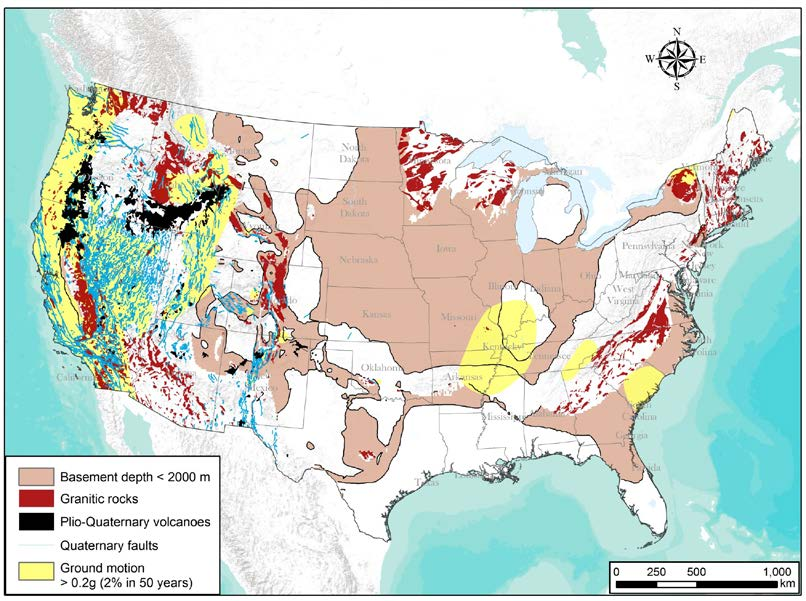
\includegraphics[width=0.8\columnwidth]{cbrock.png}	
        \caption{From \cite{Perry_2015}, a map of areas in the US with 
        crystalline basement rock at less than 2000 meters depth. Tectonic 
        activity impacting siting considerations are also mapped:  Quaternary 
        faulting, volcanism, and seismic hazard (yellow shading = 2\% 
        probability of exceeding 0.2 g in 50 years).
  \label{fig:cbrock}
\end{figure}

  
  \iffalse
  %ommitted due to lack of space
\begin{figure}[!h] 
  \centering
  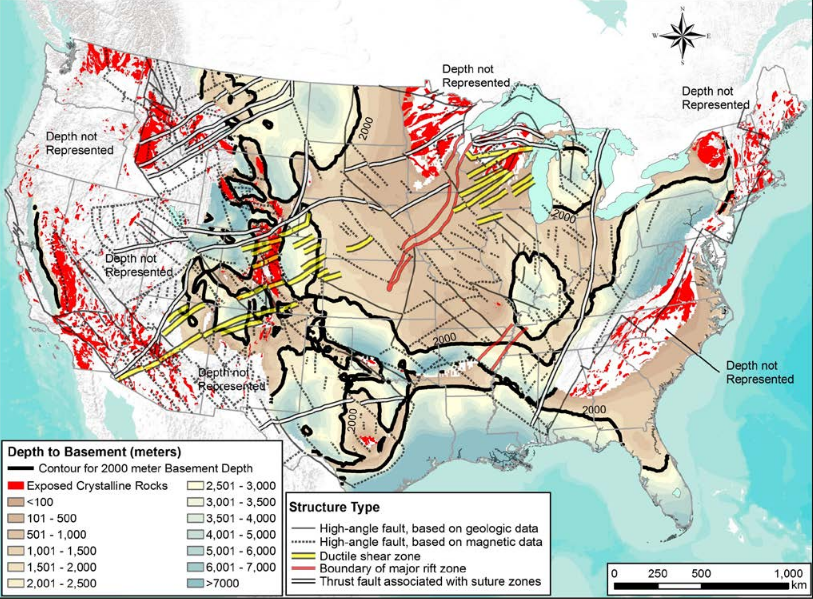
\includegraphics[width=0.8\columnwidth]{Crystalline-Thickness}	
  \caption{Depth of Crystalline Rock
  \cite{Perry_2015}.}
  \label{fig:Depth}
\end{figure}
 \fi
  
  
  Also, from the Decatur Carbon Sequestration Project, there is ample data
  on the stratigraphy of the Decatur region, which is less than 50 miles south
  of the Clinton power plant.
 
  
  
  
\begin{figure}[!h] 
  \centering
  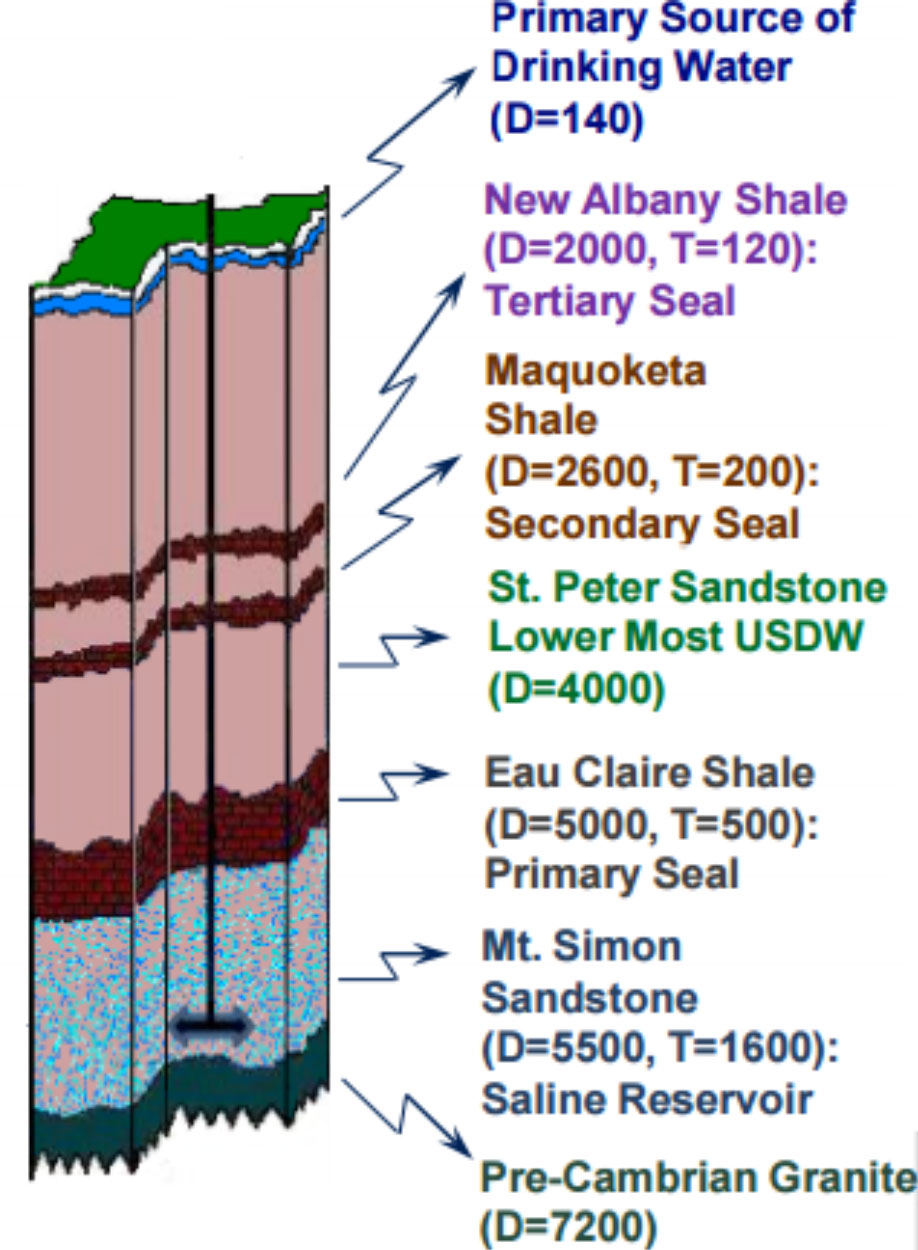
\includegraphics[width=0.8\columnwidth]{Stratigraphy-Decatur}	
  \caption{Stratigraphy of the Decatur Region
  \cite{McDonald_2012}.}
  \label{fig:Stratigraphy}
\end{figure}
  
\subsection{Base Case Methodology and Definition}
The base case is presented in order to demonstrate the cost savings and efficiencies 
that arise from the proposed case. The base case mimics the Yucca Mountain Project
but is a borehole-type repository. Costs include new licensing and processing facility
 for repacking the spent fuel assemblies.


\section {Incentives to Various Stakeholders}

Prior to discussing the benefits of the proposed case over the base case, the list of
 stakeholders and their incentives are listed below, with a number indicating the 
 magnitude of the importance of the incentive.
 
 
\begin{table}[h]

\centering
\caption {Incentive Criterion and Weight for Each Stakeholder}
\scalebox{0.65}{
	\begin{tabular}{l|l|l|l|l|l}
	\hline
	 & Federal & State & Local & Utility & Environmental \\ \hline
	Job Creation &   & 1 & 3 & 1 &   \\ \hline
	Transport[$MTHM*km$] & 2 & 1 & 2 & & 2\\ \hline
	No Need for new treatment license & 2 & & & 1 & \\ \hline
	No Need for additional land purchase & 3 & 2 & 3 & & 2 \\ \hline
	Emptying Spent Fuel Storage Pools & 3 & & & 3 & \\ \hline
	Net Cost & 3 & & & 3 & \\ \hline
	No New Above-Ground Facility Construction & 3 & & & 3 & 2\\ \hline
	
	\end{tabular}}
\end{table}

\subsection{Job Creation}

Building a spent nuclear fuel repository is no easy task. It is a task that requires
numerous experts and labourers. Also, operating and maintaining a nuclear power plant
requires numerous experts and labourers. In case of the proposed case, the Clinton
 Power Station has approximately 700 employees living in nearby counties with an
additional several hundred contractors during fuel outages\cite{Exelon}.
The existing skilled workers and local talent for maintenance, transport and catering
services can be utilized without bringing a whole new group of workers to the area \cite{IAEA_2008}. 

The base case does produce more jobs, since it needs additional constructions such
as the repackaging infrastructure. It is estimated that jobs created during the
construction was between 3,200 to 4,000 \cite{Riddel_2003}.
 However, the job creation may not be as
appreciated greatly by the local community than that of the proposed case.

Additionally, an estimate by the Illinois State University on fracking the New Albany
Shale in southern Illinois estimated that such a project can create 1,000-47,000 jobs
\cite{Loomis_2012}. Translating the workforce to central Illinois and the borehole
project should create somewhere in the low and medium estimate, which is about 10,000
jobs.

%%something about the state?


Thus, the void created by the shutdown of the Clinton plant can be, though not
completely, filled by the new construction of a borehole repository. The construction
will prioritize local hires as an incentive to ease local opposition on repository
 siting. Employment during the operation of Yucca Mountain was estimated to range from
 2,000 to 5,000 jobs, \cite{Riddel_2003} which means that the borehole repository
 would at leaste require half of the workforce for the same capacity.  

\subsection{Transport}
Transport of radioactive material is a difficult matter, and poses one of the greatest
problems in siting a repository. The proposed case, according to the crude analysis,
has the least amount of required transportation of spent fuel. Also, it is
conveniently located near the Canadian National rail line \cite{waleed_regional_2015}. 

%%% NWPA allows only "Transshipment of spent nuclear fuel to another civilian 
%%% reactor within the same utility system" [Title I, Subtitle B, Sec. 134(a)]



Conversely, siting the base case will have a $km*MTHM$ value of $209,575,157 km*MTHM$, 
which is approximately 2.7 times more than that of the proposed case. Also, %%railways?

\subsection{No Need for a New Treatment License}

%NRC license application

\subsection{No Need for Additional Land Purchase}
The proposed case has a licensed land area of approximately $58km^2$ and $20km^2$
 cooling heat sink, the Clinton Lake, with only $.6km^2$ being used for the facility.
  \cite{NRC_Clinton} This leaves enough room left for a 70,000 \gls{MTHM} borehole
  repository without additional land purchase from the public.
  
  However, the base case also does not require land purchase, for the land near 
  Yucca Mountain is part of the Nevada Test Site. 
  
  In this aspect, the 

\subsection{Emptying Spent Fuel Storage Pools }




\subsection{Net Cost}
The proposed case has a larger advantage over the base case in the sense that there
are already existing facility in regards to spent fuel handling and worker lodging 
and catering services. 
It is assumed, for the sake of argument, half of the construction cost of the
repacking facility in the base case is used to expand the existing facility in the
proposed case. 

\subsection{No New Above-Ground Facility Construction}
The proposed case, being a once-operating nuclear power plant, has the facility to 
repack the spent fuel assemblies into a disposal cask. However, this facility needs 
to be upgraded to handle a large influx of spent fuel assemblies, and should be
preferably automatic, to minimize worker exposure. The transported spent fuel
assemblies are repacked and inspected at the upgraded facility, and is sent to the
emplacement tubes for final disposal. Not having to build a new above-ground facility
should greatly increase the public perception, for it seems like there's minimal
impact.

The base case requires a new above-ground facility, which not only costs a great
amount, but also will be considered problematic to the public's eye. 


\section{Results and Discussion}
Given the current circumstances, a repository is crucial for the survival of nuclear
power. By selecting a power plant in a central location with lot of licensed land,
a repository with sizeable capacity can be built cheaper, more efficiently, and 
in a consent-based manner with the local community. 
